\documentclass{article}

% packages
\usepackage{amsmath, amsthm, thmtools, amsfonts, amssymb, luacode, catchfile, tikzducks, hyperref, ifthen}
\ifcsname c@kobocompile\endcsname
	\usepackage[a5paper, total={1072pt, 1448pt}, margin=10pt, includeheadfoot]{geometry} % set page margins
\else
	\usepackage[a4paper, margin=50pt, includeheadfoot]{geometry}
\fi
\usepackage[shortlabels]{enumitem}
\usepackage[skip=3pt, indent=0pt]{parskip}

% language
\usepackage[bidi=basic, layout=tabular, provide=*]{babel}
\ifcsname c@english\endcsname
	\babelprovide[main, import]{english}
\else
	\babelprovide[main, import]{hebrew}
	\babelprovide{rl}
\fi
%\babelfont{rm}{Libertinus Serif}
\babelfont{rm}[Renderer=Harfbuzz]{Libertinus Serif}
\babelfont{sf}{Libertinus Sans}
\babelfont{tt}{Libertinus Mono}

% style
\AddToHook{cmd/section/before}{\clearpage}	% Add line break before section
\linespread{1.3}
\setcounter{secnumdepth}{0}		% Remove default number tags from sections, this won't do well with theorems
\AtBeginDocument{\setlength{\belowdisplayskip}{3pt}}
\AtBeginDocument{\setlength{\abovedisplayskip}{3pt}}
\graphicspath{ {../images/} }

% operators
\DeclareMathOperator\cis{cis}
\DeclareMathOperator\Sp{Sp}
\DeclareMathOperator\tr{tr}
\DeclareMathOperator\im{Im}
\DeclareMathOperator\re{Re}
\DeclareMathOperator\diag{diag}
\DeclareMathOperator*\lowlim{\underline{lim}}
\DeclareMathOperator*\uplim{\overline{lim}}
\DeclareMathOperator\rng{rng}
\DeclareMathOperator\Sym{Sym}
\DeclareMathOperator\Arg{Arg}
\DeclareMathOperator\Log{Log}
\DeclareMathOperator\dom{dom}
\DeclareMathOperator\supp{Supp}
\DeclareMathOperator\var{Var}
\DeclareMathOperator\cov{Cov}

% commands
%\renewcommand\qedsymbol{\textbf{מש''ל}}
%\renewcommand\qedsymbol{\fbox{\emoji{lizard}}}
\newcommand{\Aa}[0]{\mathcal{A}}
\newcommand{\Bb}[0]{\mathcal{B}}
\newcommand{\CC}[0]{\mathbb{C}}
\newcommand{\Cc}[0]{\mathcal{C}}
\newcommand{\EE}[0]{\mathbb{E}}
\newcommand{\FF}[0]{\mathbb{F}}
\newcommand{\Ff}[0]{\mathcal{F}}
\newcommand{\Ii}[0]{\mathcal{I}}
\newcommand{\Gg}[0]{\mathcal{G}}
\newcommand{\Ll}[0]{\mathcal{L}}
\newcommand{\Mm}[0]{\mathcal{M}}
\newcommand{\NN}[0]{\mathbb{N}}
\newcommand{\Nn}[0]{\mathcal{N}}
\newcommand{\PP}[0]{\mathbb{P}}
\newcommand{\Pp}[0]{\mathcal{P}}
\newcommand{\QQ}[0]{\mathbb{Q}}
\newcommand{\RR}[0]{\mathbb{R}}
\newcommand{\Rr}[0]{\mathcal{R}}
\newcommand{\Ss}[0]{\mathcal{S}}
\newcommand{\TT}[0]{\mathbb{T}}
\newcommand{\Uu}[0]{\mathcal{U}}
\newcommand{\Vv}[0]{\mathcal{V}}
\newcommand{\Ww}[0]{\mathcal{W}}
\newcommand{\ZZ}[0]{\mathbb{Z}}
\newcommand{\acts}[0]{\circlearrowright}
\newcommand{\explain}[2] {
	\begin{flalign*}
		 && \text{#2} && \text{#1}
	\end{flalign*}
}
\newcommand{\maketitleprint}[0]{ \begin{center}
	%\begin{tikzpicture}[scale=3]
	%	\duck[graduate=gray!20!black, tassel=red!70!black]
	%\end{tikzpicture}	
	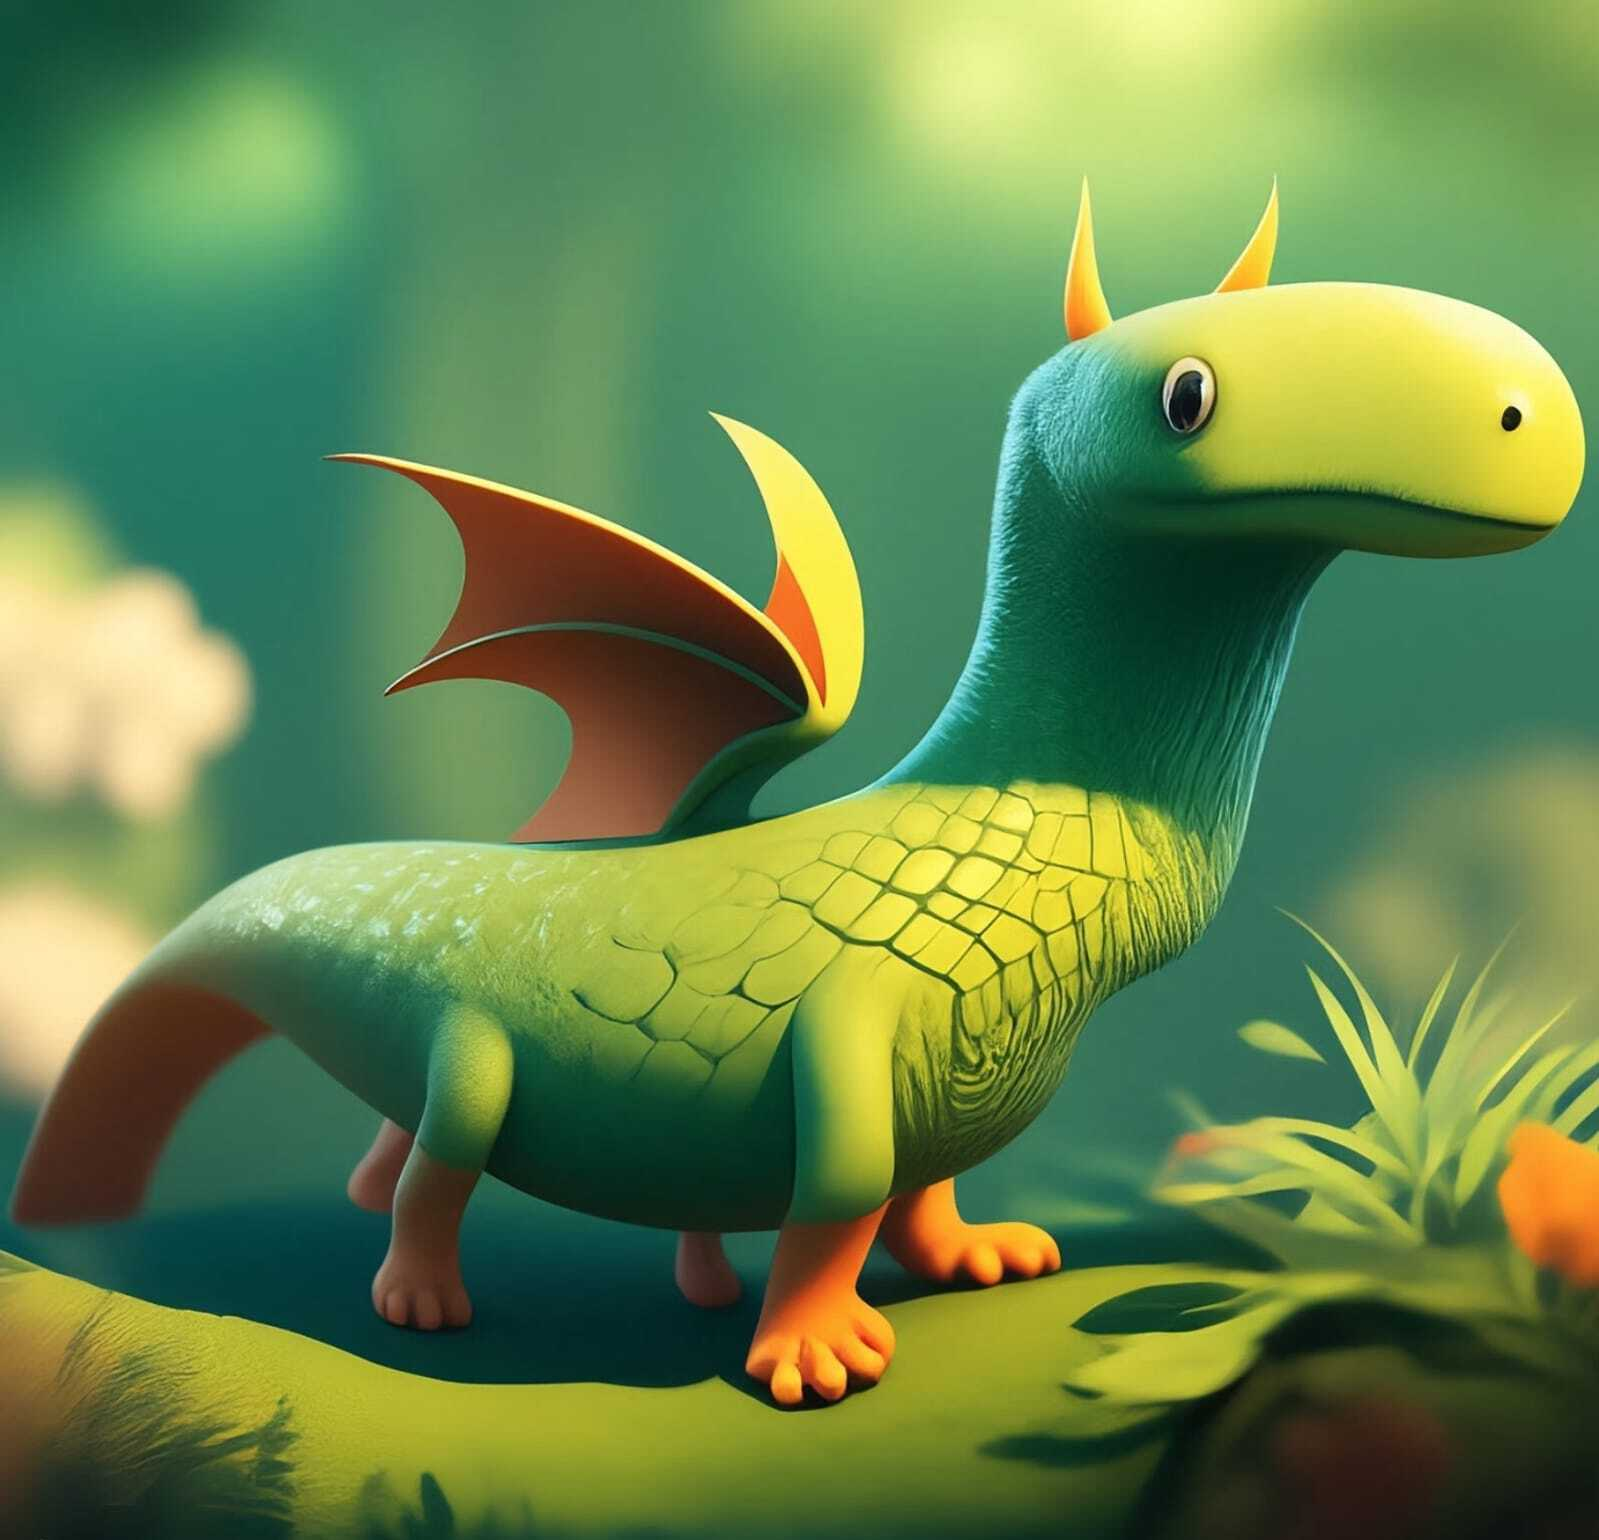
\includegraphics[width=6cm]{cover}
\end{center}
}

% theorem commands
\newtheoremstyle{c_remark}
	{}	% Space above
	{}	% Space below
	{}% Body font
	{}	% Indent amount
	{\bfseries}	% Theorem head font
	{}	% Punctuation after theorem head
	{.5em}	% Space after theorem head
	{\thmname{#1}\thmnumber{ #2}\thmnote{ \normalfont{\text{(#3)}}}}	% head content
\newtheoremstyle{c_definition}
	{3pt}	% Space above
	{3pt}	% Space below
	{}% Body font
	{}	% Indent amount
	{\bfseries}	% Theorem head font
	{}	% Punctuation after theorem head
	{.5em}	% Space after theorem head
	{\thmname{#1}\thmnumber{ #2}\thmnote{ \normalfont{\text{(#3)}}}}	% head content
\newtheoremstyle{c_plain}
	{3pt}	% Space above
	{3pt}	% Space below
	{\itshape}% Body font
	{}	% Indent amount
	{\bfseries}	% Theorem head font
	{}	% Punctuation after theorem head
	{.5em}	% Space after theorem head
	{\thmname{#1}\thmnumber{ #2}\thmnote{ \text{(#3)}}}	% head content

\ifcsname c@english\endcsname
	\theoremstyle{plain}
	\newtheorem{theorem}{Theorem}[section]
	\newtheorem{lemma}[theorem]{Lemma}
	\newtheorem{proposition}[theorem]{Proposition}
	\newtheorem*{proposition*}{Proposition}
	%\newtheorem{corollary}[theorem]{אין חלופה עברית}

	\theoremstyle{definition}
	\newtheorem{definition}[theorem]{Definition}
	\newtheorem*{definition*}{Definition}
	\newtheorem{example}{Example}[section]
	\newtheorem{exercise}{Exercise}[section]

	\theoremstyle{remark}
	\newtheorem*{remark}{Remark}
	\newtheorem*{solution}{Solution}
	\newtheorem{conclusion}[theorem]{Conclusion}
	\newtheorem{notation}[theorem]{Notation}
\else
	\theoremstyle{c_plain}
	\newtheorem{theorem}{משפט}[section]
	\newtheorem{lemma}[theorem]{למה}
	\newtheorem{proposition}[theorem]{טענה}
	\newtheorem*{proposition*}{טענה}
	%\newtheorem{corollary}[theorem]{אין חלופה עברית}

	\theoremstyle{c_definition}
	\newtheorem{definition}[theorem]{הגדרה}
	\newtheorem*{definition*}{הגדרה}
	\newtheorem{example}{דוגמה}[section]
	\newtheorem{exercise}{תרגיל}[section]

	\theoremstyle{c_remark}
	\newtheorem*{remark}{הערה}
	\newtheorem*{solution}{פתרון}
	\newtheorem{conclusion}[theorem]{מסקנה}
	\newtheorem{notation}[theorem]{סימון}
\fi

% Questions related commands
\newcounter{question}
\setcounter{question}{1}
\newcounter{sub_question}
\setcounter{sub_question}{1}

\ifcsname c@english\endcsname
	\newcommand{\question}[1][0]{
		\ifthenelse{#1 = 0}{}{\setcounter{question}{#1}}
		\section{Question \arabic{question}}
		\addtocounter{question}{1}
		\setcounter{sub_question}{1}
	}

	\newcommand{\subquestion}[1][0]{
		\ifthenelse{#1 = 0}{}{\setcounter{sub_question}{#1}}
		\subsection{Part \alph{sub_question}}
		\addtocounter{sub_question}{1}
	}
\else
	\newcommand{\question}[1][0]{
		\ifthenelse{#1 = 0}{}{\setcounter{question}{#1}}
		\section{שאלה \arabic{question}}
		\addtocounter{question}{1}
		\setcounter{sub_question}{1}
	}

	\newcommand{\subquestion}[1][0]{
		\ifthenelse{#1 = 0}{}{\setcounter{sub_question}{#1}}
		\subsection{סעיף \localecounter{letters.gershayim}{sub_question}}
		\addtocounter{sub_question}{1}
	}
\fi

% import lua and start of document
\directlua{common = require ('../common')}

\GetEnv{AUTHOR}

% headers
\author{\AUTHOR}
\date\today

\title{פתרון מטלה 03 --- מבנים אלגבריים (2), 80446}

\begin{document}
\maketitle
\maketitleprint{}

\question{}
יהי $p$ ראשוני ו־$n \in \NN$, ויהי הפולינום הציקלוטומי מסדר $p^n$,
\[
	\frac{x^{p^n} - 1}{x^{p^{n - 1}} - 1}
	\in \QQ[x]
\]

\subquestion{}
נראה שזהו אכן פולינום.
\begin{proof}
	נראה ש־$x^{p^{n - 1}} - 1 | x^{p^n} - 1$.
	ניזכר בזהות $(1 + x + \cdots + x^{n - 1})(x - 1) = x^n - 1$ הנכונה לכל $x \in \CC$.
	לכן בפרט בהצבה ${(x^{p^n})}^k - 1 = (1 + x^{p^n} + \cdots + {(x^{p^n})}^{k - 1}) (x^{p^n} - 1)$, נוכל להציב $k = p$ ונובע,
	\[
		\frac{x^{p^{n + 1}} - 1}{x^{p^n} - 1}
		= 1 + x^{p^n} + \cdots + {(x^{p^n})}^{p - 1}
	\]
	ובפרט זהו פולינום כפי שרצינו להראות.
	נבחין שעבור $n = 0$ הטענה נובעת ישירות מהזהות.
\end{proof}

\subquestion{}
נוכיח שהפולינום הוא אי־פריק על־ידי שימוש בקריטריון אייזנשטיין.
\begin{proof}
	כלל מקדמי הפולינום הם $1$ ולכן לא נוכל להשתמש בקריטריון ישירות, נציב $x = y + 1$ ונקבל,
	\[
		\frac{x^{p^n} - 1}{x^{p^{n - 1}} - 1}
		= \frac{{(y + 1)}^{p^n} - 1}{{(y + 1)}^{p^{n - 1}} - 1}
		= 1 + {(y + 1)}^{p^n} + \cdots + {(y + 1)}^{(p - 1) p^n}
		= \sum_{i = 1}^{p - 1} \sum_{j = 0}^{i p^n} \binom{i p^n}{j} y^j
		= \sum_{j = 0}^{(p - 1) p^n} \sum_{i = j / p^n}^{p - 1} \binom{i p^n}{j} y^j
	\]
	ולכן המקדם של $y^i$ הוא $\sum_{i = j / p^n}^{p - 1} \binom{i p^n}{j}$, כאשר בפרט $a_{(p - 1)p^n} = 1$, ולכן $p \mid a_i$ לכל $i < (p - 1) p^n$ אבל $p \nmid a_{(p - 1) p^n}$.
	נבחין גם כי $a_0 = p$ ולכן $p^2 \nmid a_0$, וקריטריון אייזנשטיין חל וגורר שהפולינום הציקלוטומי מסדר $p^n$ אי־פריק.
\end{proof}

\question{}
נפרק את $f(x) = x^4 + 4 \in \QQ[x]$ לפולינומים אי־פריקים מעל $\QQ$.
\begin{solution}
	נבחין כי מעל $\CC$ ל־$f$, נסמן $\omega = e^{\frac{2 \pi i}{4}} = e^{\frac{1}{2} \pi i} = \frac{1 + i}{\sqrt{2}}$, ולכן,
	\[
		f(x)
		= (x - \sqrt{2})(x - \omega \sqrt{2})(x - \omega^2 \sqrt{2})(x - \omega^3 \sqrt{2} i)
	\]
	כלומר השורשים של $f$ הם $\omega^i \sqrt{2}$ עבור $i \in \{0, 1, 2, 3\}$.
	כל פולינום $g \in \QQ[x]$ כך ש־$g \mid f$ הוא מכפלת חלק מהגורמים הלינאריים הללו, ולכן מספיק לבדוק את $2^4 - 1 = 15$ הצירופים הללו.
	כלל הפולינומים מסדר $1$ הם מכפלות של $\sqrt{2}$ ולכן נוכל להסיק ישירות שאינם פירוק של $f$ מעל $\QQ$.
	באופן דומה לא יתכן שיהיה פולינום מחלק מדרגה 3, אחרת נקבל שאיברו החופשי הוא $2 \sqrt{2} \omega_i$ עבור $i$ כלשהו.
	נותר אם כן לבדוק את 6 הפולינומים מסדר 2.
	נוכל לפסול פולינומים שלא משלימים ל־$\omega$ בחזקה זוגית, אחרת האיבר החופשי שלהם יהיה מרוכב ובפרט לא רציונלי, ונשאר לבדוק שני פולינומים בלבד,
	\[
		(x - \omega \sqrt{2}) (x - \omega^3 \sqrt{2})
		= x^2 - \sqrt{2}(\omega + \omega^3) x + 2
	\]
	אבל מתקיים,
	\[
		\omega + \omega^3
		= \frac{i + 1 + (-1 + i)}{\sqrt{2}}
		= \sqrt{2}
	\]
	ונקבל את הפולינום $x^2 - 2x + 2$.
	מבדיקה ישירה נקבל ש־$x^4 + 4 = (x^2 - 2x + 2)(x^2 + 2x + 2)$.
	עבור המקרה השני נקבל,
	\[
		(x - \sqrt{2})(x - \omega^2 \sqrt{2})
		= x^2 - \sqrt{2} (1 + \omega^2) x + 2
	\]
	כלומר המקדם של $x$ הוא $\sqrt{2}(i + 1)$ וזהו לא מספר רציונלי.
\end{solution}

\question{}
יהיו $p_1, \ldots, p_n \in \NN$ ראשוניים שונים.
נראה ש־$[\QQ(\sqrt{p_1}, \ldots, \sqrt{p_n}) : \QQ] = 2^n$ ושהקבוצה,
\[
	\Bb
	= \left\{ \sqrt{\prod_{i \in S} p_i} \middle| S \subseteq \{1, \ldots, n\} \right\}
\]
היא בסיס ל־$\QQ(\sqrt{p_1}, \ldots, \sqrt{p_n})$ מעל $\QQ$.
\begin{proof}
	אנו יודעים שמתקיים,
	\[
		[\QQ(\sqrt{p_1}, \ldots, \sqrt{p_n}) : \QQ]
		= [\QQ(\sqrt{p_1}) : \QQ ] \cdots [\QQ(\sqrt{p_1}, \ldots, \sqrt{p_n}) : \QQ(\sqrt{p_1}, \ldots, \sqrt{p_{n - 1}}) ]
	\]
	והפולינום $f_i(x) = x^2 - p_i$ מהווה פולינום מינימלי עבור כל ראשוני כזה,
	\[
		[\QQ(\sqrt{p_1}, \ldots, \sqrt{p_i}) : \QQ(\sqrt{p_1}, \ldots, \sqrt{p_{i - 1}}) ] = 2
	\]
	לכל $i$.
	נסיק אם כך ש־$[\QQ(\sqrt{p_1}, \ldots, \sqrt{p_n}) : \QQ] = 2^n$.
\end{proof}

\end{document}
